\chapter{Apps and their artefacts}~\label{chapter-apps-and-their-artefacts}
\julian{This chapter covers \uartefacts and \iartefacts. I'm currently drafting this chapter to try and work out what the major topics and groupings are, and then where the evidence I have fits. I'm currently inspired by \href{https://about.sourcegraph.com/blog/developer-productivity-thoughts}{A dev's thoughts on developer productivity}\citep{liu2022_a_devs_thoughts_onDeveloper_productivity} and the underlying spreadsheet of the findings is \href{https://docs.google.com/spreadsheets/d/1PcwJ6E_X6peCP1dBPADEAJXOBpnb4JY1gSGNyPSxedA/edit?usp=sharing}{here} and you should have access from your Google account if you are helping me with this thesis.}

The artefacts are a product, an outcome, of what developers do as they create and maintain their mobile apps. They include the source code of the codebase which evolves on an ongoing basis for active projects, any bug-tracking/bug-management system, outputs from builds including test results, outputs from mobile analytics. 

To some extent the artefacts reflect macro (big-picture) topics including ethics, scaling, data-pipelines, engineering tradeoffs, and decisions on using third-party code.


\section{Code-facing topics}



\section{Macro topics}
\subsection{Tradeoffs}
At least three types of tradeoffs were evident in the artefacts" 1) the effects of ethical decisions by the project team, 2) downgrading functionality to obtain reliability, and 3) use of third-party vs locally developed functionality. 

\textbf{Ethics}: 
Several of the development teams had to make explicit decisions whether to use mobile analytics and if so which one they would use. The Kiwix project team chose explicitly to exclude mobile analytics from their apps to reduce the potential for end users to be tracked and potentially imprisoned through their use of the app and Wikipedia content in particular~\footnote{The Kiwix project was developed to provide offline access to all of Wikipedia, it was then extended to support and provide lots of other content and material, nonetheless Wikipedia content is the one most likely to put end users at risk in some jurisdictions.} The Kiwix team did decide to use the platform-provided analytics from Google Play Console on the grounds that if the end-user had a) installed the Kiwix app from Google Play and b) had enabled (or at least not disabled) Google's collection of usage and performance data from their phones then the users were not being compromised by the devs using the analytics generated from the data those phones and tablets had provided.

The Catrobat team started by adding Fabric Crashlytics into their Pocket Code Android app several years before becoming a case study for this research. After seeing the results of applying the techniques from this research they choose to add Crashlytics to their iOS Pocket Code app and were also planning to use Firebase Analytics to record more granular usage data to both the Android and iOS apps. However, as a side-effect of migrating from the Fabric Analysis to Firebase Analysis - using the same client side SDK release they discovered they started receiving demographic data in tandem to the reliability analytics. Google then set a deadline where developers would need to replace the Fabric client side SDK with a similar one from Firebase to continue receiving any of the reports. The Catrobat team decided to stop using Crashlytics entirely rather than having demographics meta data collected by these SDKs in their apps. The Catrobat team had no objections to continuing to use the platform-provided analytics.


\textbf{Reliability trumps enhanced functionality}: 
The core Kiwix Android app included a custom file downloader that downloaded material such as Wikipedia in German for offline use. This downloader kept track of partial downloads and also allowed end users to control when to allow the downloads and when to pause or stop them. This functionality was designed to help users often in areas with intermittent, controlled, and sometimes expensive connectivity to increase their chances of being able to download the content within their budget. To provide some concrete examples in some parts of the world users would download content that took several entire \emph{days} even if the connection didn't fail, and the cost of the connection was metered and capped to 1GB of data.

However, the code for the downloader had various bugs and flaws including several that caused the app to crash. These crashes meant the app had an excessively high crash rate in the Google Play App Store. The then lead developer for the Android codebase had not been able to tame the high crash rate. A consultant was hired who had worked on multiple other Android projects and codebases. This consultant proposed scrapping the custom downloader and replacing it with standard Android functionality provided by Google as part of the Android SDK. This proposal was accepted and implemented\pending{Add details of the release and commits} and it had the desired effect of reducing the crash rate of the core Kiwix Android app by about a third\pending{check details and revise accordingly}. So far, so good.

However the standard Android downloader didn't provide equivalent facilities to continue partial downloads, or to pause and resume downloads, nor did it provide progress tracking information. Furthermore as the project team had chosen not to incorporate in-app mobile analytics the project team cannot easily determine the effects of these changes \emph{on the end users}. Bugs continue to surface occasionally on the project's GitHub site~\footnote{\textit{e.g.} \url{https://github.com/kiwix/kiwix-android/issues/2845}.} and users sometimes complain in reviews submitted to Google Play. Here are four examples extracted from the developer's view of Google Play:

\begin{itemize}
    \item ``\textit{Wikipedia nopic without images works again in version 11.18 with search function.! Top Unfortunately, now in March 21 again problems with wikipedia text with 14.2 gb. After 3/4 of the download the process breaks off every time! Too bad. Wikis with smaller amounts of data can be downloaded without any problems. Handling of the app very well.}'', Mar 22, 2021 % https://play.google.com/console/u/0/developers/9116215767541857492/app/4975184706939091905/user-feedback/review-details?reviewId=gp%3AAOqpTOGjPB5Em_o1TfLCzltkR7jvVhdVJAvBZlj9Y0-5i9FOcDaJ4Yjh1yqIHV5-qo-9HkbvGJSAHweXJOQodfo&corpus=PUBLIC_REVIEWS
    \item ``\textit{Download started and it could never finish}'', Mar 25, 2021 % https://play.google.com/console/u/0/developers/9116215767541857492/app/4975184706939091905/user-feedback/review-details?reviewId=gp%3AAOqpTOErPflFJDpyqiz4m4CJW3IPjYoXKGrO0SLZ4L94DwUPj662lAWuS0MOWAXfANZ2D6Vf--EkJLe1RPIeSqk&corpus=PUBLIC_REVIEWS
    \item ``\textit{Seems that library download is b0rken atm?}'', Oct 7, 2021 % https://play.google.com/console/u/0/developers/9116215767541857492/app/4975184706939091905/user-feedback/review-details?reviewId=gp%3AAOqpTOGVOb-MNO3ehakCJsUi7Ur-R_6QJkdnWzFDl7xh6KA28ZUATGKmBO7JzDTgPvULR0UhivkWMp2B0d83qpA&corpus=PUBLIC_REVIEWS
    \item ``\textit{Cant continue interrupted download}'', Oct 15, 2021 % https://play.google.com/console/u/0/developers/9116215767541857492/app/4975184706939091905/user-feedback/review-details?reviewId=gp%3AAOqpTOFxVKQVzPIrgcWHmCX8QnQXaqVkI8JFVwBzLYiDHJrdBbokV8SBDfRRjYltEqBp8lsLVTNFlix3fzFMHYA&corpus=PUBLIC_REVIEWS
\end{itemize}

And another review asks for the download manager that, ironically, used to exist (presumably without realising the app used to have one): ``\textit{edit: still there is no download manager. It is not possible to download the large files. Despite 100 megabits per second, I did not manage to load the large Wikipedia with images. The app itself is very good. Only the download of the huge files always breaks off. I load via PC. A download manager would not be bad.}'', Mar 12, 2021 % https://play.google.com/console/u/0/developers/9116215767541857492/app/4975184706939091905/user-feedback/review-details?reviewId=gp%3AAOqpTOEH9rOv2WWhAUTEChRwgT1Mrq5rYxEp9cQzrqjGDg6aeOccjVgxJeNFU_syr1wNPh9UMw71FKfM13iNy8k&corpus=PUBLIC_REVIEWS 

The third tradeoff is between third-party and locally developed code which generalises the second tradeoff found in the research (of trading functionality for reliability). As a concrete example, the WebView component is ubiquitous on Android and found in many Android apps including several of those in the case study\pending{Is it worth the investment to find out how many of the apps use the Android WebView?}. 

% Google's overview on the WebView component is available at https://developer.android.com/guide/webapps and https://developer.android.com/guide/webapps/webview-privacy discusses crash reporting and other data collection topics pertaining to apps using WebViews.

As projects, including the Kiwix team, discovered crashes can be reported in Android Vitals for the WebView component. These adversely affect the app's reliability as measured by Android Vitals. While the app developers can fix at least some of the causes of third-party components, including the WebView component, others may be beyond their direct control.

In March 2021, major apps including apps from the Amazon, BBC, Facebook, Google, Microsoft, etc. failed in use by a release of the WebView component~\citep{peters2021_google_fixes_issue_causing_android_apps_to_crash_etc_webview, bbcnews2021_google_fixes_crashing_android_app_issues, bbc_iplayer_app_april_2021_webview_information}. and Samsung's bland observation % https://www.samsung.com/ph/support/mobile-devices/google-webview-issue/ 
All their respective app developers relied on a third-party software component developed and maintained by Google as part of Android. Furthermore, app developers who have incorporated the WebView into their app sometimes introduced bugs in their use of the WebView. Across a population of 146 opensource Android apps 124 WebView related bugs were found and the root causes analysed~\citep[pp. 704 - 706]{hu2018_a_tale_of_two_cities_how_webview_introduces_bugs_to_android_applications}. Of these bugs, 15 introduced crashes~\citep[p. 706]{hu2018_a_tale_of_two_cities_how_webview_introduces_bugs_to_android_applications}.

As Google Android notes online \url{https://developer.android.com/guide/webapps} there are various alternatives to using a WebView. They don't mention either a) developers developing their own user interface, or b) other third-party alternatives to their WebView (\emph{e.g.} \href{https://mozilla.github.io/geckoview/}{Mozilla's GeckoView}). 
% https://stackoverflow.com/questions/35559467/webview-alternatives (the answer is too dated to include in my thesis). and https://www.i-programmer.info/news/193-android/12900-the-geckoview-alternative-to-webview.html 
% https://android.gadgethacks.com/how-to/ditch-googles-webview-switch-androids-system-browser-bromite-0384227/ 

There is no silver bullet for developers in terms of choosing whether to write their own code or use third-party code. Tradeoff 2 enabled the Kiwix team to improve the reliability at the cost of losing functionality; tradeoff 3 allows developers to short-circuit the work of developing their own functionality at the risk of being unable to address some of the failures and problems related to using those third-party components.


\section{Normal and acceptable ranges of failures}
For the GTAF case study, the crash rates, as measured by Android Vitals, vary massively by release of the app (Al Quran (Tafsir \& by Word).\pending{A great deal more analysis is possible given the number of active apps and the ongoing access to Google Play Console.} 

Android Vitals does not report any failures in the GTAF taskinator app, which is created using React Native according to the development team. This is pertinent as similar behaviours in Android Vitals were observed for another app-centric case study, LocalHalo. 


\section{Improvements in crash rates}
For both Catrobat and Kiwix the hackathon and the post-hackathon bug fixes were highly effective in terms of cumulatively reducing the crash rate over several subsequent releases. % TODO Check whether the releases were contiguous.
The Catrobat case study replicated the improvements seen in the Kiwix case study and also the efficacy of using a hackathon as an immediate intervention. TODO discuss limitations of hackathons and forward link to the section on the useful half-life of hackathons. 


For Pocket Code, the improvements in the stability of the app were particularly encouraging as the project had already implemented many of `good' development practices.


\section{Discussion}\label{apps-and-artefacts-discussion-section}
Much of a developer's focus, perhaps unsurprisingly, is working with code and modifying code to achieve various objectives. An industry-focused article by Beyang Liu discusses the author's thoughts on developer productivity and introduces a term `\textbf{developer hertz}' as a measure of developer productivity~\citep{liu2022_a_devs_thoughts_onDeveloper_productivity} and defines it as once around the developer's inner loop (illustrated in Figure \ref{fig:developer-inner-loop-outer-loop}). This article provides a helpful context for the work of app developers where automated tests, use of mobile analytics, bug reproducibility, bug tracking, choosing third-party libraries, and various other activities emerged from the thematic analysis of the various findings pertaining to this research.

\begin{figure}
    \centering
    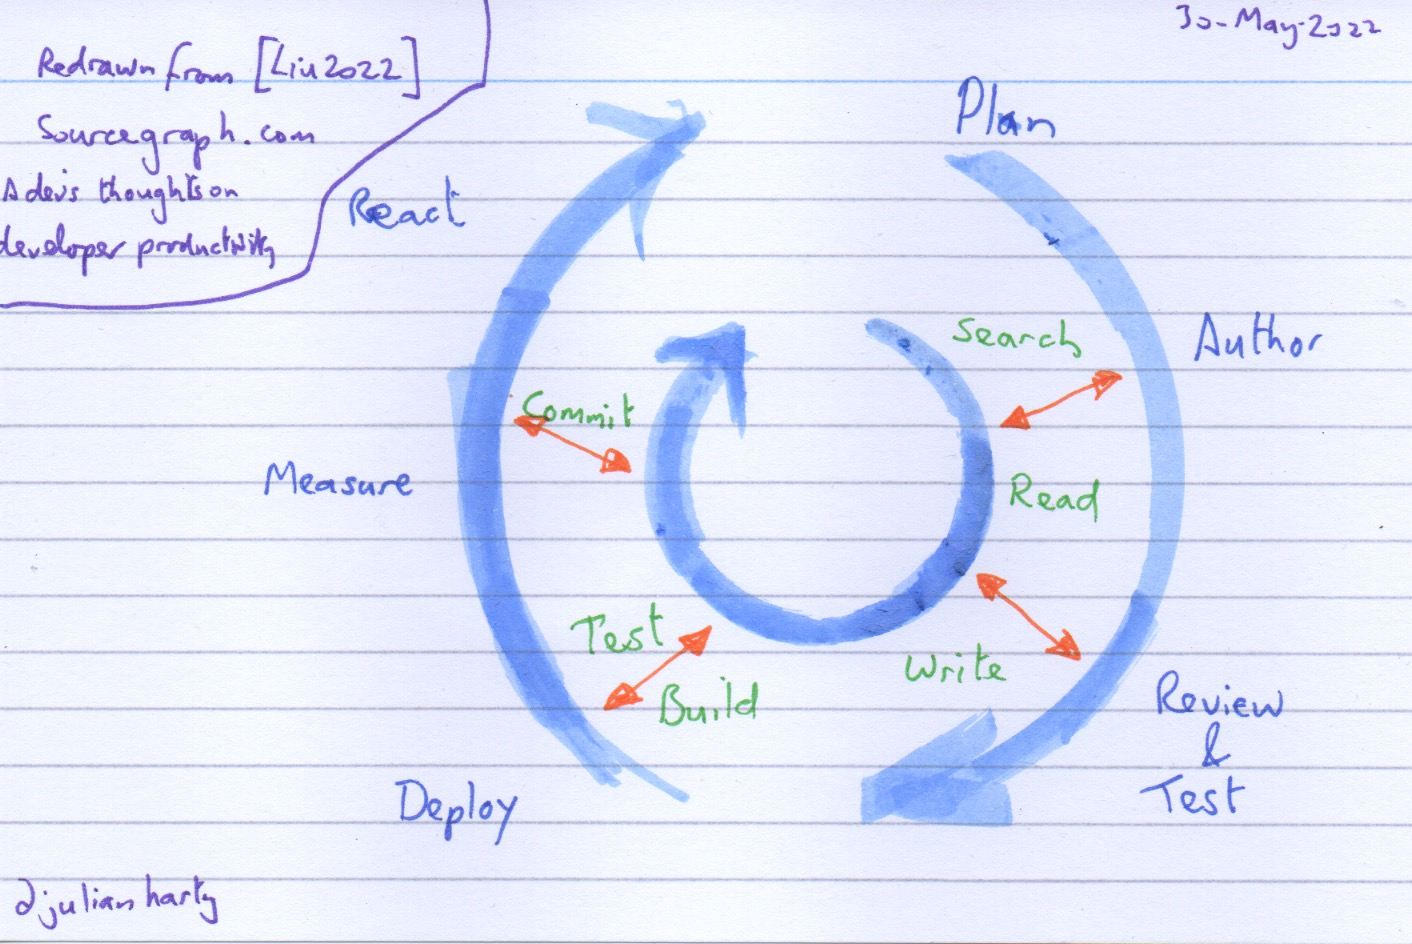
\includegraphics[width=12cm]{images/rough-sketches/developer-inner-loop-outer-loop.jpeg}
    \caption{Developer Inner Loop, Outer Loop\\ redrawn from \citep{liu2022_a_devs_thoughts_onDeveloper_productivity}}
    \label{fig:developer-inner-loop-outer-loop}
\end{figure}

\subsection{An iterative development lifecycle for app developers}
The research includes many findings that illustrate a conceptual iterative loop for app developers in terms of how their code is performing; to answer how's it doing in the real world. Figure \ref{fig:dev-app-reliability-iterative-loop} approximates various potential activities within this loop.

\begin{figure}
    \centering
    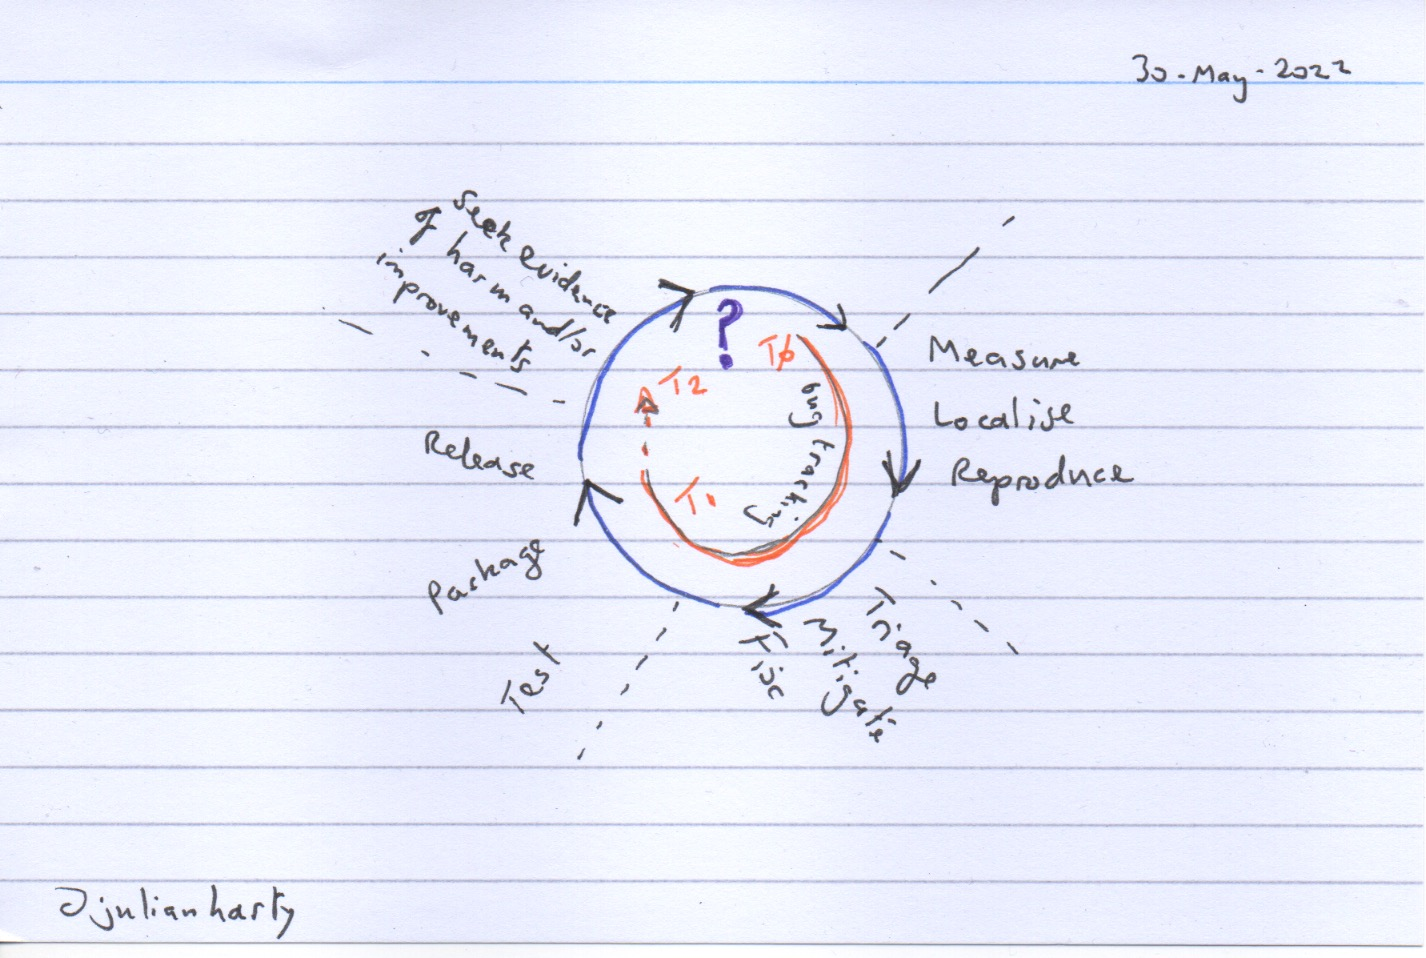
\includegraphics[width=12cm]{images/rough-sketches/dev-app-reliability-iterative-loop.jpeg}
    \caption{Developer's conceptual app reliability iterative loop}
    \label{fig:dev-app-reliability-iterative-loop}
\end{figure}

The loop starts with at the question-mark where the developers have a question about a flaw in the field related to their app's performance. They search for information which may include bug-localisation, adding logging to the app, and trying to reproduce the flaw using various techniques. They \emph{may} record the flaw in their issue tracking system, if so T0 marks the start of that bug in the bug tracking system.

They \emph{may} triage, mitigate, and/or attempt to fix the flaw, and if so they are likely to test the potential improvement(s), package the changes in a potential release and release it via the app store. Once the new release starts to be deployed they can start to seek evidence for any new/additional harm and/or any improvements in the performance of the app.

If the developer recorded the bug in the reporting system there are two more potential points of transition; T1 is when the developer believes the issue has been addressed for instance through modifications to the source code of the app, and T2 would be if there is evidence from the mobile analytics that the changes had the desired results. \emph{Not all teams/developers seek or record T2}.


\section{Summary of apps and their artefacts}
TBC